\ifdefined\AuthorVersion
\documentclass[manuscript,screen]{acmart}
\else
\documentclass[manuscript,screen,review,anonymous]{acmart}
\fi
\setcopyright{none}
\settopmatter{printacmref=false}
\acmJournal{DTRAP}
\acmDOI{}
\usepackage{amsmath,booktabs,tabularx,array,graphicx,placeins}
\setlength{\emergencystretch}{2em}
\newcommand{\F}{\textsc{Frozen}}
\newcommand{\FIT}{\textsc{Fit192}}
\newcommand{\CAL}{\textsc{Role64}}
\newcommand{\code}[1]{\texttt{\detokenize{#1}}}
\newcommand{\pp}{\,\mathrm{pp}}
\newcommand{\meanauc}{\overline{\mathrm{AUC}}_{\mathrm{block}}}
\makeatletter
\newcommand{\tablerows}[1]{\@@input #1 }
\makeatother

\title{Thresholds and Learning in Adaptive Intrusion Detection: A Two-Capture Case Study}
\ifdefined\AuthorVersion\author{Oleksandr Kuznetsov}
\orcid{0000-0003-2331-6326}
\authornote{Corresponding author.}
\email{oleksandr.kuznetsov@uniecampus.it}
\affiliation{\department{Department of Theoretical and Applied Sciences}\institution{eCampus University}\city{Novedrate}\country{Italy}}
\affiliation{\department{SMARTEST Research Center}\institution{eCampus University}\city{Novedrate}\country{Italy}}
\affiliation{\department{Department of Intelligent Software Systems and Technologies, School of Computer Science and Artificial Intelligence}\institution{V. N. Karazin Kharkiv National University}\city{Kharkiv}\country{Ukraine}}
\author{Emanuele Pio De Bernardis}
\orcid{0009-0004-7915-5204}
\email{emanuelepio.debernardis@gmail.com}
\affiliation{\department{Department of Theoretical and Applied Sciences}\institution{eCampus University}\city{Novedrate}\country{Italy}}
\author{Emanuele Frontoni}
\orcid{0000-0002-8893-9244}
\email{emanuele.frontoni@unimc.it}
\affiliation{\department{Department of Political Sciences, Communication and International Relations}\institution{University of Macerata}\streetaddress{Via Crescimbeni, 30/32}\city{Macerata}\postcode{62100}\country{Italy}}
\renewcommand{\shortauthors}{Kuznetsov et al.}
\newcommand{\setauthorpdfmetadata}{\hypersetup{pdfauthor={Oleksandr Kuznetsov; Emanuele Pio De Bernardis; Emanuele Frontoni}}}
\else\author{Anonymous Authors}\fi
\begin{document}
\begin{abstract}
Threshold selection and calibration coverage can change conclusions about adaptive intrusion detection even when label acquisition is fixed. We develop an auditable evaluation procedure and apply it to chronological TON\_IoT and UNSW-NB15 captures under sparse, delayed supervision. Paired controls separate score refitting, calibration capacity, label eligibility, and update timing. On TON\_IoT, a frozen spline detector targeting 5\% calibration false-positive rate (FPR) attains 31.98\% future FPR when calibration is restricted by a permanent feature-vector role. Calibration on all acquired labels reduces this to 4.53\% under the same update schedule. Recurrent normal vectors are concentrated in a few types, and errors accumulate on types excluded from calibration. Refitting still supplies a conditional benefit when both scores use the same all-label memory: at false-positive cost weight two, balanced accuracy is 87.94\% for the head and 86.78\% for the frozen score, with 3.22 percentage points lower FPR and 0.89 points lower recall. At 13\% FPR, paired interpolation gives a recall difference of $3.06\pm3.02$ points. The head's all-label controller nevertheless attains 10.22\% FPR at the 5\% target. On UNSW-NB15, historical frozen policies remain stronger by balanced accuracy. Five seeds describe variation conditional on each stream; role-partition and memory sensitivity substantially exceed the default seed variation. The contribution is a reproducible evaluation procedure that locates error trade-offs and calibration failure, with explicit limits on what these two captures establish.
\end{abstract}
\ccsdesc[500]{Security and privacy~Intrusion detection systems}
\ccsdesc[300]{Computing methodologies~Machine learning}
\keywords{intrusion detection, delayed labels, calibration coverage, threshold selection, error trade-offs, reproducibility}
\maketitle
\ifdefined\AuthorVersion\setauthorpdfmetadata\fi

\section{Introduction}
An intrusion detector assigns a score to each observation and compares it with a decision threshold. Updating the score and moving the threshold are different interventions. Either can change the number of missed attacks and false alarms. A comparison of adaptive and static detectors therefore needs controls that identify which score, threshold, and calibration-data interventions supply the reported improvement.

This question becomes more difficult when labels are scarce and delayed. The observations available for refitting may differ from those available for threshold selection. A small calibration memory can favor a different operating point from a larger memory, even when both optimize the same objective. Furthermore, a frozen model can be a weak reference because its initial fit transfers poorly to the evaluation period. These effects can make a large adaptive-versus-frozen contrast misleading as evidence of general learning superiority.

We study these issues using chronological TON\_IoT and UNSW-NB15 replays. The principal question is: \emph{what improvement remains after specifying a strong threshold-only controller, a relevant operating point, and a clear label-use contract?} The model families are an additive spline detector, logistic regression (LR), and an adaptive random forest (ARF). The spline intervention refits only eight feature gains and an intercept, providing a compact, explicit change to the score function.

The contribution is a reproducible evaluation procedure and a case study containing both positive and negative results: paired score and memory interventions, causal threshold selection, explicit label-use contracts, baseline-quality audits, and representation recurrence analysis. The results below emphasize operating policies and baseline quality. The Supplement retains the full historical campaign, implementation details, attack-family results, resource accounting, and sensitivity tables.

\section{Related work}
Concept-drift research distinguishes changes in a data-generating process from the mechanisms used to detect or respond to them \citep{gama2014}. Prequential evaluation requires prediction before an observation is used for learning \citep{gama2013}; delayed-label evaluation makes the feedback schedule explicit \citep{grzenda2020}. Adaptive random forests combine online ensembles with drift-triggered replacement \citep{gomes2017}. Active learning addresses the separate question of which labels to request \citep{zliobaite2014}. We use uniform requests so that acquisition remains fixed across controllers.

In security, INSOMNIA combines adaptation with active learning and label estimation \citep{andresini2021}; continuous Android malware learning similarly couples representation updates and selective labeling \citep{chen2023}. Transcend and CADE study drift detection and explanation \citep{jordaney2017,yang2021}. Our focus is the downstream attribution of decision changes once feedback is available. Temporal and spatial biases, deployment assumptions, and dataset construction remain central to this interpretation \citep{pendlebury2019,arp2022,sommer2010,engelen2021}.

Threshold selection differs from probability calibration \citep{guo2017}. Here CAL denotes examples used to select a binary threshold, without asserting that scores are posterior probabilities. Prior-shift correction provides an intercept-based reference \citep{saerens2002,lipton2018}, while changing class-conditional traffic can require more than an intercept. The spline score is a logistic generalized additive model \citep{hastie1986}; its fixed univariate representation also relates to neural additive models and KANs \citep{agarwal2021,liu2025}. The study evaluates update policies rather than proposing a new architecture.

\section{Data and causal evaluation}
\subsection{Captures, partitions, and feature availability}
TON\_IoT supplies network records from a controlled IoT/IIoT environment \citep{moustafa2021,booij2022}. We retain eight complete-flow numerical features: duration, source/destination bytes, missed bytes, and source/destination packet and IP-byte counts. Records are ordered by start time plus duration. A fits the initial transformation and model, B selects historical thresholds, C supports the original development, and D is evaluated. The full dates, preprocessing counts, and earlier structural exposure are recorded in Supplement S1.

UNSW-NB15 supplies a separately collected laboratory capture \citep{moustafa2015unsw,moustafa2016unsw}. We use its four full network CSVs, remove only three verified duplicate file-boundary rows, and retain 2,540,044 records. The eight numerical fields are \code{dur}, \code{sbytes}, \code{dbytes}, \code{sloss}, \code{dloss}, \code{Spkts}, \code{Dpkts}, and \code{tcprtt}. This is a compact feature contract with different semantics from TON. Records are sorted by $\max(\mathrm{Ltime},\mathrm{Stime}+\mathrm{float32}(\mathrm{dur}))$, then stable row identity, and split chronologically 40\%/20\%/40\% into A/B/D. Equal timestamps at boundaries are retained without an embargo. Models are fitted anew on each dataset.

\begin{table}[tb]
\centering\small
\caption{Evaluation streams. Observed prevalence is retained. Each dataset supplies one recorded stream, shared by all five algorithmic seeds.}
\label{tab:data}
\begin{tabular}{lrrrr}
\toprule
Stream & D records & Normal & Attacks & Hours \\
\midrule
TON\_IoT & 3,549,973 & 309,673 & 3,240,300 & 62.77 \\
UNSW-NB15 & 1,016,018 & 803,736 & 212,282 & 7.89 \\
\bottomrule
\end{tabular}
\end{table}

\subsection{Models, feedback, and memory}
All models use a fixed $\log(1+\max(x,0))$ transformation and standardization fitted on A. The initial LR and spline fits use the same seeded 400,000-row sample of A. LR uses the eight transformed inputs. The spline model fits eight cubic B-spline basis coefficients per feature, with subsequent adaptation restricted to
\begin{equation}
 s(x;g,b)=b+\sum_{j=1}^{8}g_j f_j(x_j),
\end{equation}
where the eight functions $f_j$ remain fixed. A head update fits eight gains and an intercept by regularized logistic regression on the current FIT memory. The original refit uses zero-centred L2 regularization; a previous-head-centred alternative is retained in the Supplement.

The stream is predicted in 10,000-row blocks. Uniform requests select 1\% of each block without replacement. Requested labels from block $k$ arrive after prediction of block $k+1$ and first affect block $k+2$. The last incomplete block is retained. All methods use the same requested row identities within a dataset, seed, delay, and budget condition. The current sampler uses \code{SeedSequence([seed, block, 20261101])}. The archived campaign's older sampler is used only in its separate numerical bridge.

A salted hash of each raw feature vector assigns it permanently to FIT or CAL with nominal probabilities 3/4 and 1/4. The default memories hold 192 FIT and 64 CAL observations, with equal class quotas for eviction; one class can occupy the other class's unused slots. Repeated observations can occupy separate positions. CAL entries are eligible for 50 blocks from observation time; at least five observations of each class are required. FIT has no age filter. A head and its matched threshold change atomically only when the transaction is valid. We name memories by eligibility and capacity: \textbf{ROLE64} and \textbf{ROLE256} accept only CAL-role observations; \textbf{ALL256} accepts every acquired label. ALL256 thresholds update whenever their own class minimum is met. The suffix \textbf{-G} instead applies the successful head-transaction gate. These names apply throughout the paper and Supplement. The head always fits FIT192. Head/ALL256 therefore reuses some fitting labels for threshold selection, while ROLE memories preserve feature-vector disjointness.

\begin{table}[tb]
\centering\small
\caption{Information contracts. All rows share acquisition and feedback timing. Model state and pending labels are additional to the listed example memories.}
\label{tab:contracts}
\begin{tabularx}{\linewidth}{lXX}
\toprule
Controller & Learning & Threshold selection \\
\midrule
Frozen / B & A only & Historical B \\
Frozen / ALL256 & A only & All acquired labels; own class-minimum gate \\
Head / ROLE64 & Disjoint FIT192 & ROLE64; valid head transaction \\
Frozen/head / ROLE256 & A only or fixed FIT192 trajectory & Same ROLE256 and head gate \\
Frozen/head / ALL256 & A only or fixed FIT192 trajectory & Same ALL256 and own gate; fitting-label reuse for head \\
Frozen/head / ALL256-G & Same scores as above & Same ALL256 and head gate \\
ARF / ROLE64 or ALL256 & Every arriving requested label & CAL labels reused in learning \\
ARF FIT-only / ROLE64 & Arriving FIT-role labels only & Disjoint ROLE64 \\
\bottomrule
\end{tabularx}
\end{table}

ARF uses River 0.22.0, ten trees, and defaults apart from the seed \citep{riverdocs}. The first extension processes the A sample chronologically. The present audit additionally fits the identical sample in its seeded random order. Both initial states are evaluated frozen and with feedback. The FIT-only variant starts from the chronological state and excludes every CAL-role label from learning. This aligns label disjointness with the head experiment, while retaining the forest's persistent tree memory. It does not impose the finite FIT192 retention contract. Thus ARF is an equal-acquisition-budget comparator with explicitly different model state and, for its standard variant, different label reuse.

\subsection{Controls with identical calibration observations}
The original Frozen/ALL256 versus Head/ROLE64 contrast changes score learning, calibration capacity, label eligibility, and the threshold-update gate. It estimates a complete policy-package difference. To isolate the score intervention, we cross frozen and adapted scores with CAL-role capacities 64 and 256 on both streams and all five seeds. Within each capacity, the two scores use exactly the same labeled occurrences, age filter, objective, tie rule, and update times. Both CAL buffers remain disjoint from FIT192 and use the default role salt.

The head follows the original FIT192/ROLE64 trajectory in every cell. All four thresholds change only at successful transactions of that trajectory. Thus increasing CAL capacity changes threshold evidence while holding the fitted score sequence and its gate fixed. ROLE256 retains up to 448 FIT+CAL observations in total, compared with 256 for FIT192/ROLE64, without extra label requests. It is a controlled memory intervention, rather than a fully retuned 448-example learner. Every shared per-block prediction count and threshold agrees exactly with the retained earlier replay.

\subsection{All-label and eligibility controls}
An additional ten replays hold the original head trajectory fixed and calibrate both frozen and head scores on the identical ALL256 observations, at identical times. Both scores also receive ALL256-G thresholds. Comparing ALL256 and ALL256-G isolates the schedule; comparing ALL256-G and ROLE256 holds capacity and schedule fixed while changing label eligibility. No extra labels are acquired. Head/ALL256 has a more permissive label-use contract than the disjoint head: its calibration includes labels used to fit the score. Evaluation still predicts future observations before using their labels.

We audit the role assignment directly on all normal D vectors, for the default salt and the two previously declared alternatives. The summaries distinguish the fraction of unique vectors assigned to CAL from their occurrence-weighted traffic mass. We also sum false positives separately over CAL-role and FIT-role normal observations. These strata identify where calibration exclusions and errors coincide.

\subsection{Threshold objectives and matched-error descriptions}
A decision is positive when $s(x)>\tau$. The historical and recent thresholds minimize
\begin{equation}
 L_\lambda(\tau)=\mathrm{FNR}(\tau)+\lambda\,\mathrm{FPR}(\tau).
 \label{eq:cost}
\end{equation}
The first extension fixes $\lambda\in\{0.25,0.5,1,2,4\}$; the current audit adds 0.75, 1.25, 1.5, and 3. Every threshold is fitted using past available labels. At $\lambda=1$, this is equivalent to maximizing balanced accuracy (BA). Exact candidate and tie rules appear in Supplement S1. For attack prevalence $\pi$ and costs $C_{\rm FN},C_{\rm FP}$, the rate weight is $C_{\rm FP}(1-\pi)/(C_{\rm FN}\pi)$. A value of one is a declared evaluation objective, rather than a universal operational cost.

Two complementary checks address operating-point comparability. First, we interpolate the observed FPR/recall polylines within their support, separately for each paired seed. This is a retrospective description of recorded policies. It neither selects a deployable threshold nor estimates an oracle ROC curve. Interpolating a curve of seed means is also reported and kept distinct from averaging the paired-seed comparisons.

Second, causal FPR-target controllers use only past normal calibration scores. For target $\alpha\in\{0.05,0.10,0.20\}$, they select the smallest observed negative-score threshold with empirical FPR at most $\alpha$, respecting complete ties. B supplies the initial threshold. The original package comparison uses ALL256 for the frozen score and disjoint ROLE64 for the head. The matched-memory audit also evaluates both scores on identical ROLE64 and ROLE256. Requested targets are identical; achieved future FPR can differ under distribution change. We report both achieved FPR and recall rather than assuming that a calibration target is a future guarantee.

\subsection{Metrics, overlap, and evidence status}
We sum confusion counts over D before calculating recall, FPR, BA, and precision. AUROC and noninterpolated average precision (AP) are also calculated within prediction blocks containing both classes. We report macro, normal-count-weighted, and attack-count-weighted summaries and their coverage. Pooled AUROC/AP are used only for a fixed score. Pooling adaptive scores would compare values from different fitted states. AP is the recall-increment-weighted mean of precision, as implemented by scikit-learn, rather than a trapezoidal interpolation \citep{pedregosa2011,sklearnap}.

Seen/unseen strata refer to exact equality of eight stored float32 features against earlier A/B/C vectors on TON and A/B vectors on UNSW. They describe representation recurrence, not event identity, attack-family novelty, or memorization. Both strata are evaluated on the same adaptive trajectory.

\subsection{Scope of claims}
Each dataset supplies one recorded capture. Seeds 42--46 vary initial sampling and label requests; every mean and sample SD is conditional on that stream and the stated controller configuration. Salt and memory changes are reported separately. TON diagnostics were designed after D outcomes were examined, and UNSW had appeared elsewhere in the project; all extensions are exploratory. Within replay, thresholds and scores use only past feedback. Across the research process, these are case studies of two controlled captures. They do not estimate performance across operational networks.

Policy-package contrasts, score interventions with matched threshold evidence, retrospective interpolation, and causal target controllers answer distinct questions. An interpolated point describes recorded policies within their common support; a calibration target describes the selection rule, whose future error is measured separately. Feature recurrence denotes exact equality of the stored inputs, not event identity or a causal estimate of memorization. ARF shares acquisition but retains persistent trees and may reuse calibration labels in learning. These conventions apply to all Results and Supplement tables.

The historical empirical rule required joint non-increase of FN and FP, with at least one strict improvement, in four of five spline seeds against Frozen/ROLE64. It is a versioned acceptance criterion rather than a significance test. Counts for other learners and comparators are exploratory.

\subsection{Computational assistance and verification}
OpenAI ChatGPT/Codex was used under the corresponding author's direction to assist with diagnostic protocol formulation, implementation, execution of replay scripts, numerical analysis, and plotting (November 2026 sessions). The exact backend model snapshot was not retained. Reproducibility is based on the archived executable source, fitted initial states, pinned numerical environment, input digests, per-block reports, and deterministic analysis scripts. Figures are generated from recorded numerical outputs with Matplotlib. The matched-memory audit verifies 274,090 replay checks and 1,930 analysis checks. The additional all-label audit verifies 600,825 replay checks and 574,280 source, trajectory, and aggregation checks. Shared predictions, thresholds, label requests, and head-state digests agree exactly across the diagnostic implementations. AI assistance is a tool-use disclosure; responsibility for scientific interpretation and the submitted work rests with the human authors.

\section{Results}
\subsection{Permanent roles can exclude normal traffic from calibration}
The main failure is visible in Table~\ref{tab:coverage}: at a 5\% calibration target on TON, Frozen/ROLE64 and Frozen/ROLE256 attain 31.54\% and 31.98\% future FPR. Frozen/ALL256 attains 4.57\%. Increasing role-memory capacity does not repair this gap. With the same head-transaction gate, Frozen/ALL256-G attains 4.53\%, so the update schedule explains little of this particular difference. At $\lambda=2$, changing from ALL256-G to ROLE256 increases frozen FPR from 13.08\% to 32.80\%.

\begin{table}[tb]
\centering\small\setlength{\tabcolsep}{4pt}
\caption{Achieved future FPR at three calibration targets. Entries are percentages, averaged over the five seeds; complete recall, BA, and seed SDs are in Supplement S7. ALL accepts all acquired labels; ROLE accepts only the permanent CAL role.}
\label{tab:coverage}
\begin{tabular}{lr rrr rrr}\toprule
& & \multicolumn{3}{c}{Frozen score} & \multicolumn{3}{c}{Head score}\\
Stream & Target & ALL256 & ROLE64 & ROLE256 & ALL256 & ROLE64 & ROLE256\\\midrule
\tablerows{tables/calibration_target_rows.tex}
\bottomrule\end{tabular}
\end{table}

The role audit explains why capacity and coverage are different. TON contains 87,132 distinct normal D vectors among 309,673 normal observations; 73.94\% of observations belong to repeated vectors. The ten most frequent vectors account for 46.23\% of normal traffic. Because the role is a function of the vector, every occurrence of a FIT-role type is permanently excluded from ROLE calibration. About 25\% of unique normal vectors receive the CAL role under each salt, but their traffic mass ranges from 17.59\% to 35.22\%; the default is 31.05\%.

At the default 5\% target, Frozen/ROLE256 has 42.87\% FPR on FIT-role normals versus 7.80\% on CAL-role normals. The corresponding head rates are 11.80\% and 9.92\%. The head therefore reduces errors primarily in the excluded population under this policy, while slightly worsening the included population. This supports the diagnosis of calibration-selection failure and a compensating score intervention. It does not establish that all head benefit is caused by role exclusion: the all-label control below retains a learning effect. Nor does total CAL mass alone predict quality; Salt 2 has less CAL traffic mass and a better default head result than the default salt.

\begin{figure}[tb]
\centering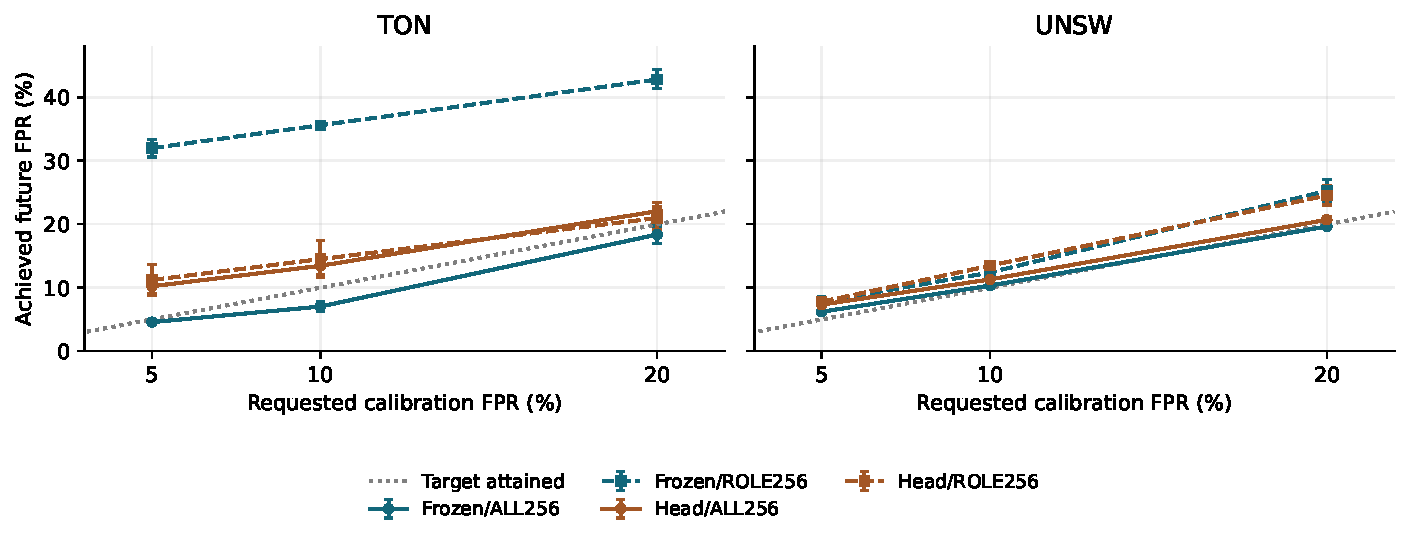
\includegraphics[width=\linewidth]{figures/calibration_eligibility.pdf}
\caption{Requested versus achieved FPR with frozen and head scores on ALL256 or ROLE256. Bars show conditional seed SD; the dotted line marks target attainment. Axes are identical. Changing calibration eligibility substantially changes TON's frozen controller; head target violations persist with ALL256.}
\Description{Two panels plot requested FPR of five, ten and twenty percent against achieved FPR for TON and UNSW. TON frozen role calibration is far above the target line; all-label calibration brings the frozen detector near or below that line. The head exceeds the five-percent target even with all labels.}
\label{fig:eligibility}
\end{figure}

\subsection{Score changes under identical all-label calibration}
Table~\ref{tab:allscore} supplies the missing common-calibration comparison. At $\lambda=1$ on TON, Head/ALL256 versus Frozen/ALL256 changes FPR by $-30.19\pm5.12$ percentage points and recall by $-0.21\pm0.71$. At $\lambda=2$, the differences shrink to $-3.22\pm1.16$ and $-0.89\pm2.56$, respectively; BA increases by $1.16\pm0.87$ points. Both scores use the same observations, capacity, update times, objective, and tie rule. The ALL256-G pairs yield the same score contrasts. Thus the large contrast at one cost weight is not solely an artifact of role-restricted calibration, but its magnitude depends strongly on the threshold objective.

\begin{table}[tb]
\centering\small\setlength{\tabcolsep}{3pt}
\caption{Frozen and head scores with identical ALL256 calibration and update times. Rates are percentages, mean $\pm$ conditional seed SD. The head reuses fitting labels for calibration; this permissive contract is separate from the disjoint ROLE controls.}
\label{tab:allscore}
\begin{tabular}{lr rrr rrr}\toprule
& & \multicolumn{3}{c}{Frozen/ALL256} & \multicolumn{3}{c}{Head/ALL256}\\
Stream & $\lambda$ & Recall & FPR & BA & Recall & FPR & BA\\\midrule
\tablerows{tables/all_label_score_rows.tex}
\bottomrule\end{tabular}
\end{table}

At 13\% FPR, within-seed interpolation of these all-label cost policies gives head-minus-frozen recall $3.06\pm3.02$ points across all five TON pairs; at 20\%, it gives $3.23\pm1.58$. The 10\% target has only four supported pairs and a wider $13.70\pm9.95$-point difference. On UNSW, Head/ALL256 has lower BA than Frozen/ALL256 at both $\lambda=1$ and 2, and both remain below historical spline Frozen/B. The all-label head is therefore an informative diagnostic of score changes, not a general replacement for a frozen policy.


\subsection{Score changes persist when calibration memory is matched}
Table~\ref{tab:samememory} separates score changes from CAL capacity. At $\lambda=1$ on TON, the head-minus-frozen difference with identical ROLE64 is $-28.15\pm5.22$ percentage points in FPR and $-1.91\pm2.33$ in recall. With identical ROLE256, the corresponding differences are $-28.94\pm4.89$ and $-1.56\pm2.37$. A score intervention therefore changes the error compromise under this fixed role and calibration policy; unequal memory is not the sole explanation of the original contrast.

Increasing head calibration capacity from 64 to 256, while retaining the same head trajectory, adds $1.83\pm0.51$ BA points at $\lambda=1$ on TON and $0.59\pm0.22$ on UNSW. On UNSW, however, the score contrast itself changes from $-0.54\pm0.39$ BA points at ROLE64 to $+0.30\pm0.24$ at ROLE256, and both remain below historical Frozen/B. This interaction cautions against describing a head-learning benefit without its calibration contract.

\begin{table}[tb]
\centering\fontsize{9}{10.5}\selectfont\setlength{\tabcolsep}{2.4pt}
\caption{Matched calibration observations and update times. CAL is the capacity of the disjoint CAL-role memory. The FIT192 head trajectory is held fixed. Rates are percentages, mean $\pm$ conditional seed SD; $\lambda$ is the FP weight.}
\label{tab:samememory}
\begin{tabular}{lrr rrr rrr}\toprule
& & & \multicolumn{3}{c}{Frozen score} & \multicolumn{3}{c}{Head score}\\
Stream & CAL & $\lambda$ & Recall & FPR & BA & Recall & FPR & BA\\\midrule
\tablerows{tables/diagnostic_b_same_memory_rows.tex}
\bottomrule\end{tabular}
\end{table}

The label-eligibility contract matters beyond capacity. On TON at $\lambda=2$, frozen ROLE256 yields 32.80\% FPR and 76.80\% BA, whereas ALL256 yields 13.16\% FPR and 86.78\% BA. These memories have the same nominal capacity but different eligible observations and update gates. The larger role-restricted memory does not recover the all-label controller's behavior. The role audit in Section~4.1 identifies the excluded population and its errors; the gated all-label controls distinguish eligibility from update timing. Supplement S6 provides the complete same-memory target controllers, operating curves, supported matched-error descriptions, and per-seed counts.

\subsection{The apparent head benefit depends on threshold policy}
The complete-policy table in Supplement S7 compares the original complete policy packages against the stronger all-label threshold-only control. On TON at $\lambda=1$, Head/ROLE64 has 28.36 percentage points lower FPR and 2.92 points lower recall than Frozen/ALL256. Each seed has fewer FP and more FN. 

Changing only the frozen detector's cost weight to $\lambda=2$ raises its BA from 72.12\% to 86.78\%, above the head's 84.84\% at $\lambda=1$. At $\lambda=2$, the head reaches 87.55\% BA. The large 28-point FPR contrast therefore describes one objective and information contract, rather than a comparable advantage across operating points. The intermediate frozen weight $\lambda=1.25$ gives 87.22\% BA, illustrating the sensitivity to this choice without establishing that a weight selected after inspecting D will transfer. The observed operating curves in Figure~\ref{fig:costs} show where the gap changes.



\begin{figure}[tb]
\centering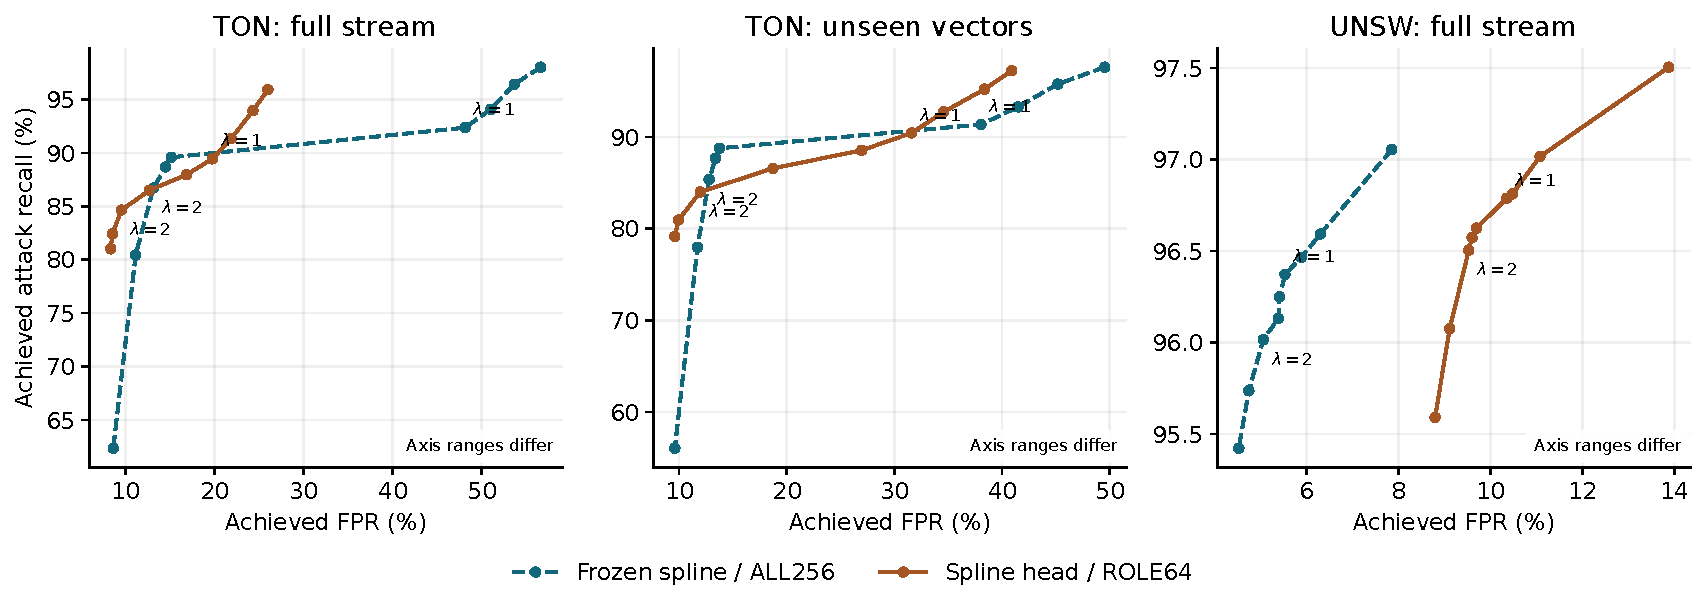
\includegraphics[width=\linewidth]{figures/diagnostic_a_operating_points.pdf}
\caption{Causal threshold policies for the fixed cost grid. Points are means over five paired randomizations on each single stream. Lines connect implemented policies and do not constitute an oracle frontier. Axis ranges differ. The annotated weights illustrate why a single $\lambda=1$ contrast cannot establish curve-wide superiority.}
\label{fig:costs}
\Description{Causal threshold policies for the fixed cost grid. Points are means over five paired randomizations on each single stream. Lines connect implemented policies and do not constitute an oracle frontier. Axis ranges differ. The annotated weights illustrate why a single $\lambda=1$ contrast cannot establish curve-wide superiority.}
\end{figure}

The original five-point grid also makes interpolation resolution important. In TON seed 42, the frozen thresholds at $\lambda=0.25$ and 0.5 coincide in 238 of 355 blocks; those at 2 and 4 coincide in 201. Finite calibration data produce shared thresholds and coarse operating points. Supplement S4 provides each seed and distinguishes interpolation of the mean curve from paired-seed interpolation. The latter retains variation in the location of the operating points; the two summaries need not agree.

The earlier mixed comparison, Head/ROLE64 versus Frozen/ALL256, gives $1.49\pm3.66$ recall points at 13\% FPR. Its different calibration contract distinguishes it from the ALL256 comparison above.

On UNSW, the historical Frozen/B spline is strongest by mean BA among the default spline policies: 96.29\%. Recent ROLE64 selection lowers BA to 93.75\%, ALL256 to 95.42\%, and head/ROLE64 to 93.22\%. Thus neither tested recent threshold adaptation nor head refitting improves BA over the historical policy on this capture. A higher recall under another policy remains possible at a larger false-alarm cost. This qualifies any claim that adaptation generally fails or succeeds independently of the chosen utility.

\subsection{Calibration targets and precision--recall}
The complete target table in Supplement S7 evaluates common calibration FPR targets. These controllers supply a causal check independent of the $\lambda=1$ objective. Their realized FPRs must be examined before comparing recall: the same calibration target can produce different future false-alarm burdens. In particular, a small ROLE64 sample and a changed score can miss the requested target substantially.



At the nominal 20\% target on TON, Head/ROLE64 has 91.50\% recall versus 80.53\% for Frozen/ALL256, a difference of 10.97 points. Their achieved FPRs are 19.95\% and 18.37\%, respectively: this supports a useful comparison in a nearby operating region, not an exactly matched-FPR estimate. At targets 5\% and 10\%, Head/ROLE64 produces FPRs of 12.07\% and 16.03\%. ROLE256 gives 11.21\% and 14.49\%; ALL256 gives 10.22\% and 13.44\%. Neither larger role memory nor reuse of all labels attains these TON targets. At the 20\% target, Head/ALL256 reaches 94.08\% recall with 22.04\% FPR. The frozen all-label target controller attains lower FPR with lower recall. The small paired interpolation difference near 13\% FPR supports operating-region dependence, not statistical equivalence or absence of benefit at every lower FPR. In fact, the earlier five-weight interpolation at 10\% uses only four supported pairs and is more variable. Target-based policies and cost-weight interpolation describe different sets of operating policies.

The $\lambda=1$ contrast alone cannot diagnose sampling noise as the cause. On TON, weighting valid calibration/next-block pairs by the next block's normal count gives calibration FPR 42.67\% and subsequent FPR 48.30\% at $\lambda=1$, versus 8.26\% and 13.20\% at $\lambda=2$. Thus the selected calibration policy already accepts many false alarms; the subsequent rates also reflect transfer. The diagnostic supplement compares calibration and subsequent-block errors and records the number of distinct normal scores. These measurements separate a policy that accepts many false alarms in its calibration objective from one that violates an intended FPR target after transfer. They do not identify a unique causal source of the observed shift.

\subsection{Baseline quality changes the interpretation of learning}
The frozen LR on TON has pooled D AUROC 0.318 and Frozen/B BA 25.50\%. We therefore audited attack-label orientation, the coefficient score, \code{decision_function}, attack probabilities, optimization convergence, and the cached score. The fixed-score A/B/D diagnostics are in Table~\ref{tab:audit}. An inversion on B or D is an observed transfer failure; it is not repaired by reversing scores using D labels. Consequently, the poor frozen LR is retained as a failure case rather than presented as a strong performance comparator.

\begin{table}[tb]
\centering\small
\caption{Initial-model audit: pooled AUROC, mean $\pm$ seed SD conditional on each capture. A describes the training population and is not an out-of-sample estimate. The chronological and shuffled forests use the same sampled A rows.}
\label{tab:audit}
\begin{tabular}{llrrr}\toprule
Stream & Initial model & A & B & D \\\midrule
\tablerows{tables/diagnostic_a_audit_rows.tex}
\bottomrule\end{tabular}
\end{table}

Against its own Frozen/ALL256 control, the TON LR head reduces FP in all five seeds and FN in four. The exception is seed 45, with 62,138 additional FN. This is an exploratory 4/5 joint-improvement count for a different learner and comparator; it does not overturn the failed historical spline criterion. Its interpretation also depends on the frozen LR's poor ranking. Similar head BA values for LR and splines conceal different starting points and error changes.

The initial chronological forest is also weak. On UNSW, seed 43 has a constant score, AUROC 0.5, and recall and FPR of 100\% at the historical threshold. Three other seeds have inverted pooled ranking. TON's frozen forest has pooled AUROC 0.40--0.46. Large adaptive-versus-frozen differences against these states cannot alone establish the superiority of a richer learner. Table~\ref{tab:arf} therefore includes the shuffled-A initialization and the disjoint-label feedback control, while retaining the original chronological results.

\begin{table}[tb]
\centering\fontsize{8.7}{10.5}\selectfont\setlength{\tabcolsep}{3pt}
\caption{Forest diagnostics, percentages as mean $\pm$ SD across five randomizations conditional on each capture. All policies share acquired labels; FIT-only uses a subset for learning and disjoint ROLE64. Tree state is persistent and is not constrained to the head's example-memory contract.}
\label{tab:arf}
\begin{tabular}{lllrrr}\toprule
Stream & Initial/feedback condition & Policy & Recall & FPR & BA \\\midrule
\tablerows{tables/diagnostic_a_arf_rows.tex}
\bottomrule\end{tabular}
\end{table}

For the original chronological initialization, adaptive ARF/ALL256 reaches 90.39\% BA on TON, compared with 86.78\% for spline Frozen/ALL256 at $\lambda=2$ and 87.55\% for the spline head at $\lambda=2$. On UNSW it reaches 95.86\%, close to spline Frozen/ALL256 at $\lambda=1$ (95.42\%) and below spline Frozen/B (96.29\%). The standard ARF uses all acquired labels for learning, reuses CAL labels, and retains persistent tree state.

On TON, shuffled-A ARF/ALL256 reaches 89.94\% BA; its corresponding frozen/ALL256 state reaches 73.67\%, and its historical frozen/B policy reaches 57.78\%. The chronological FIT-only/ROLE64 forest reaches 87.43\%, using CAL-role labels exclusively for threshold selection.

On UNSW, shuffled-A ARF/ALL256 reaches 96.74\% BA; its corresponding frozen/ALL256 state reaches 96.94\%, and its historical frozen/B policy reaches 97.84\%. The chronological FIT-only/ROLE64 forest reaches 94.32\%, using CAL-role labels exclusively for threshold selection.

At 20\% FPR, within-seed interpolation of the shuffled forests' nine-weight policies gives adaptive-minus-frozen recall $18.24 \pm 13.88$ percentage points across all five supported pairs. This comparison uses adaptive ROLE64 versus frozen ALL256, and the forest retains persistent state and calibration-label reuse. It supports a TON learning contribution under that contract beyond the spline-specific single-point contrast. The selected matched-FPR targets have no common support for all five UNSW pairs; no extrapolated forest comparison is used there.

These initialization and label-use contrasts delimit the forest result. The shuffled initial state is a batch-initialization control on historical A, not a reshuffling of the evaluation stream. The FIT-only control removes calibration-label reuse during D while preserving the forest's accumulated tree state; it supplies a label-use check rather than an equal-memory comparison.


\begin{figure}[tb]\centering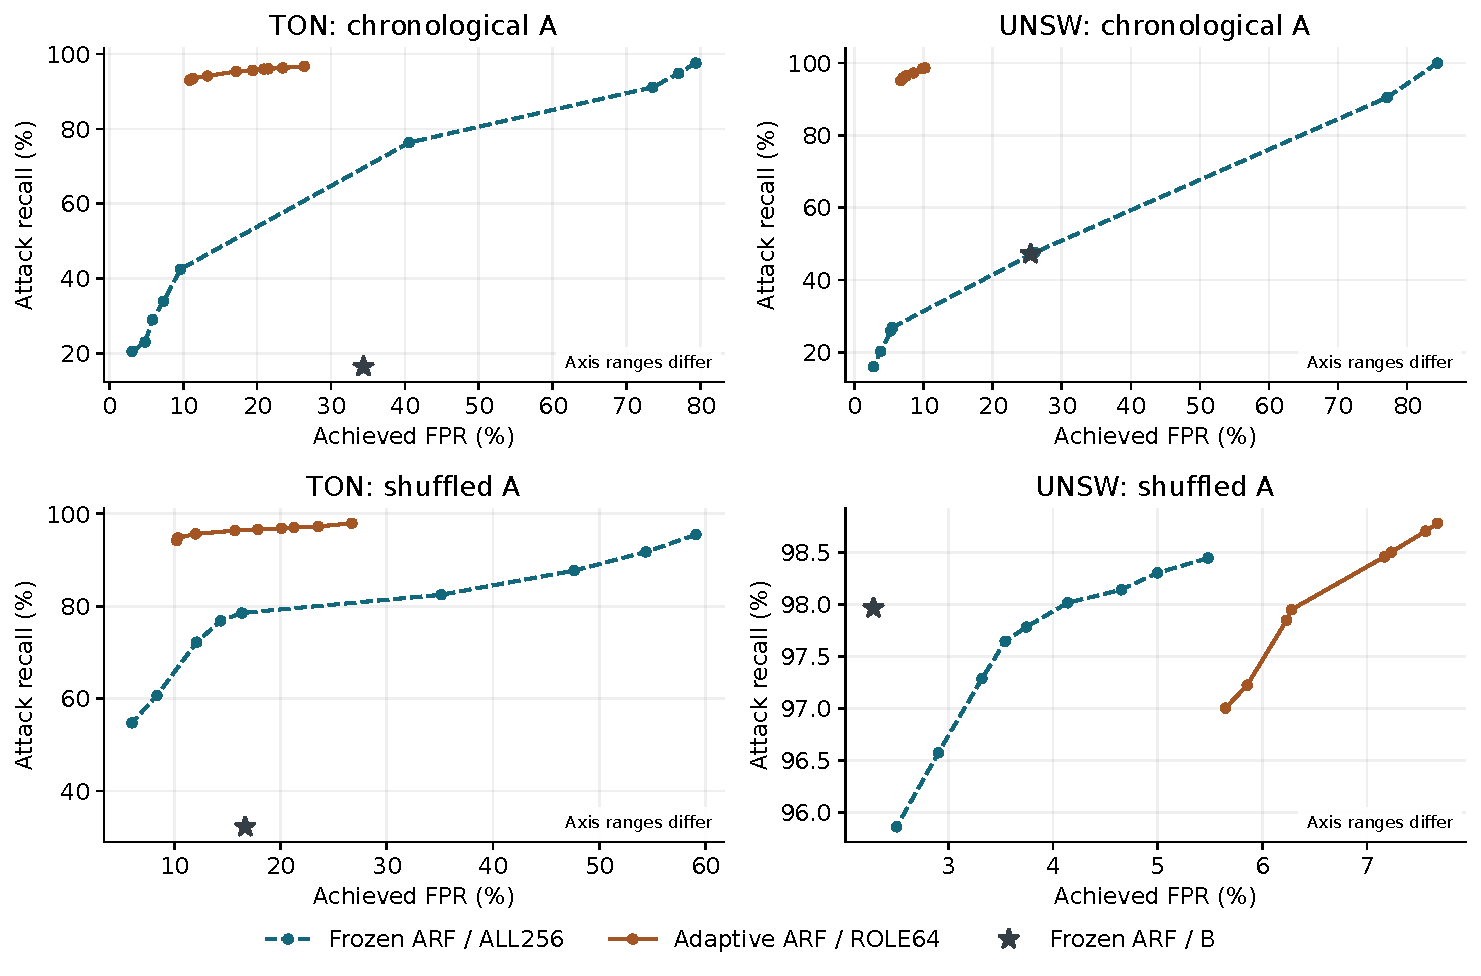
\includegraphics[width=\linewidth]{figures/diagnostic_a_forest_operating_points.pdf}
\caption{Forest operating policies under chronological and shuffled historical initialization. Connected points use the nine fixed cost weights, with thresholds selected from past labels. Stars mark the fixed historical B threshold. Means describe five randomizations on each stream; axis ranges differ. The frozen control uses ALL256 and the adaptive forest ROLE64; the standard forest reuses CAL labels for learning and retains persistent tree state.}
\label{fig:forest}
\Description{Forest operating policies under chronological and shuffled historical initialization. Connected points use the nine fixed cost weights, with thresholds selected from past labels. Stars mark the fixed historical B threshold. Means describe five randomizations on each stream; axis ranges differ. The frozen control uses ALL256 and the adaptive forest ROLE64; the standard forest reuses CAL labels for learning and retains persistent tree state.}
\end{figure}
Figure~\ref{fig:forest} places the forest comparisons in their operating regions. The historical-threshold point can outperform recent calibration on stable ranking, while an adaptive policy can help after poor transfer. A comparison at one weight, including an ARF comparison, remains a statement about the specified complete policies. The Supplement's CSV includes paired matched-error descriptions for these forests as well.


\subsection{Ranking heterogeneity and controller sensitivity}
The frozen spline's TON macro block AUROC is 0.850, while weighting valid blocks by their normal counts gives 0.557. Blocks with few normal observations have disproportionate influence on the macro summary relative to their contribution to false-alarm workload. The normal-weighted statistic exposes weak average within-block separation under that weighting. The false-alarm workload therefore needs the normal-weighted summary alongside macro AUROC and achieved FPR. Both summaries, pooled fixed-score AUROC, blockwise AP, and coverage are retained in Supplement S4.

Controller robustness is assessed one factor at a time on both captures: FIT/CAL capacities 96/32 and 384/128; calibration ages 10 and 100 blocks; a minimum of ten CAL examples per class; and two additional fixed role salts. All five seeds are retained for every setting. These checks assess the declared controller rather than selecting a new best configuration. They complement the earlier TON delay and budget tests: at a 0.1\% query budget the default spline head reaches 57.49\% BA, compared with 79.48\% for Frozen/ALL256. Detailed rates, update counts, and conditional variation are reported in the Supplement.

On TON, head BA across the eight declared settings ranges from 81.49\% to 88.97\%. The default and the two alternative role salts yield 84.84\%, 83.95\%, and 88.97\%, respectively. On UNSW, head BA across the eight declared settings ranges from 89.63\% to 93.89\%. The default and the two alternative role salts yield 93.22\%, 92.44\%, and 89.63\%, respectively.

The default TON seed SD is only 0.79 BA points. It conditions on one chosen role salt and memory configuration, whereas the 81.49--88.97\% range changes those choices. Neither quantity is a confidence interval for performance on a new stream. The three fixed salts give separate TON means of 84.84\%, 83.95\%, and 88.97\%; their within-salt SDs are 0.79, 1.50, and 1.41 points. Supplement S6 reports all salts separately. Three deterministic partitions do not estimate a population distribution over arbitrary salts, and the one-factor checks do not estimate joint configuration uncertainty. The observed salt dependence is substantial and differs between captures. A favorable individual partition should therefore not be reported as a stable model advantage. Across these eight head settings, UNSW BA remains below the historical frozen spline.

\subsection{Historical Stage 1 and its numerical sensitivity}
The archived TON campaign established the original motivation. With a frozen score, recent ROLE64 raises recall from 21.11\% to 89.09\%, while FPR rises from 12.64\% to 46.74\%. Adding head refitting gives recall 89.38\% and FPR 20.47\%. Of the FP reduction, 96.7\% occurs on vectors previously observed in A/B/C, where recall decreases. The full-stream FN mean combines opposing seen/unseen changes. Only seeds 43, 45, and 46 improve both error counts, so the specified 4/5 criterion fails.

The same-query Linux numerical bridge changes that count from 3/5 to 2/5. Its paired FN differences are $+33{,}457$, $-115{,}004$, $+123{,}984$, $-45{,}794$, and $+47{,}576$ for seeds 42--46, respectively. The seed-46 change is largely associated with its frozen calibration trace. This sensitivity is evidence against treating a seed-count cutoff as an inferential conclusion. The original measurements remain historical evidence; the bridge is a separately fitted reconstruction, not bitwise replication. Full counts and provenance appear in Supplement S2--S3.

\section{Discussion and limits}
The complete-policy comparison and the matched-memory audit answer different questions. The former compares usable policy packages under a common acquisition budget; the latter isolates the effect of changing the score under identical threshold evidence and timing. Equal $\lambda$ comparisons are meaningful tests of two specified calibration procedures, but they cannot establish uniform superiority of their score functions. Matched-error descriptions and causal FPR-target controllers answer complementary questions. A strong evaluation should report the operating region, actual achieved rates, effective calibration evidence, and the quality of the frozen reference.

The overlap result is similarly conditional. The first extension's $\lambda=1$ spline comparison locates 90.5\% of FP savings on previously seen vectors. This percentage describes where that policy saves false alarms. It is not the fraction of benefit caused by memorization, and it changes when the control or operating objective changes. Exact feature equality can merge distinct flows and miss near-duplicates. A tolerance-based or host/session analysis would require a separately justified identity definition; it is outside the present eight-feature recurrence claim.

A useful next design assigns FIT/CAL roles per queried occurrence using a fixed independent randomization. This preserves disjoint observations while allowing repeated feature types to appear in both roles. It changes the current feature-vector-disjoint contract, so recurrence and near-duplicate dependence must still be measured. Cross-fitting or rotating holdouts are other possible designs. Their calibration behavior requires a new prospective experiment; the present diagnostics motivate these tests rather than validate a repair.

Feedback is also an assumption. At the 1\% budget, TON requires approximately 566 labels per recorded hour and UNSW approximately 1,288. Block-delay medians are about 3.50 and 6.45 minutes, respectively. These volumes and delays describe an annotation service, not a demonstrated analyst workflow. Labels are treated as correct. Active acquisition, noisy or asynchronous analyst feedback, and operational capacity estimation require new experiments. A deployment-specific $\lambda$ should be set from past evidence and declared costs or capacity, with an evaluation period kept separate.

Reproducibility has two levels. Original Windows reports are preserved and reanalyzed exactly, while the available Linux reconstruction does not reproduce every initial fit or prediction. The new extensions retain initial models, source hashes, input-array digests, full per-block reports, and pinned dependencies so that their recorded analyses and causal replays can be checked. A Git revision identifies the implementation; the archival package preserves the evidence and its provenance.

\section{Conclusions}
Calibration eligibility is a consequential part of an adaptive intrusion detector. On TON, a permanent feature-role partition excludes recurring normal types from threshold selection. A frozen detector targeting 5\% FPR then incurs about 32\% future FPR with either ROLE64 or ROLE256, compared with about 4.5\% on ALL256 under the same update schedule. Capacity alone cannot correct a missing population.

Score refitting partly compensates for that exclusion, and a conditional score benefit also survives common all-label calibration. At $\lambda=2$, Head/ALL256 improves TON BA by $1.16\pm0.87$ points over Frozen/ALL256; at 13\% FPR the paired recall difference is $3.06\pm3.02$ points. Head target violations persist, and UNSW favors historical frozen policies. These results locate the benefit in a stated calibration contract and operating region.

The highest-BA tested policies on both captures retain the historical B threshold: adaptive shuffled ARF/B reaches 94.37\% on TON and frozen shuffled ARF/B reaches 97.84\% on UNSW; historical frozen spline reaches 96.29\% on UNSW. This motivates retaining a historical-threshold control before replacing it with a small recent sample. It is a comparison of the tested policies, not a universal rule for choosing B.

The resulting evaluation procedure matches score comparisons on calibration observations and timing, separates capacity from eligibility, checks achieved target errors, audits initial models, and reports partition sensitivity alongside conditional seed variation. Its value is an auditable account of when an apparent adaptive gain survives stronger controls and where calibration failure changes its interpretation.

\section*{Data and code availability}
TON\_IoT and UNSW-NB15 are used under their providers' academic-use conditions \citep{toniotweb,unswweb}; raw network records are not redistributed. The reproducibility package contains source attribution, reconstruction instructions, fitted initial states, per-block reports, tabular summaries, and executable checks. The article and Supplement build directly from the recorded evidence; replaying predictions requires separately obtained source data.
\ifdefined\AuthorVersion
The versioned reproduction package is archived on Zenodo at \url{https://doi.org/10.5281/zenodo.23880240}; the public implementation and article sources are also available from the \href{https://github.com/KuznetsovKarazin/kan-ids-v2/tree/paper2/dtrap-submission-20261102}{article branch}. The release manifest identifies the source revision, historical execution sources, and neutral diagnostic sets A--C.
\else
An anonymized numerical-evidence package accompanies the manuscript. Source provenance and the full reproduction package are supplied separately to the editors to preserve double-anonymous review.
\fi

\ifdefined\AuthorVersion
\section*{Author contributions and declarations}
\noindent\textbf{CRediT authorship contribution statement.} Oleksandr Kuznetsov: Conceptualization, Methodology, Formal analysis, Investigation, Software, Validation, Visualization, Supervision, Project administration, Writing---original draft, Writing---review and editing. Emanuele Pio De Bernardis: Software, Investigation, Data curation, Validation, Visualization, Writing---original draft, Writing---review and editing. Emanuele Frontoni: Funding acquisition, Project administration, Writing---review and editing. De Bernardis developed the original implementation and experimental campaign. Kuznetsov directed the additional diagnostic protocols, computational analyses, and manuscript revision; the computational assistance used for the extensions is described in Methods.

\noindent\textbf{Funding and acknowledgements.} GAIA S.r.l., a spin-off of the University of Macerata, supported Emanuele Pio De Bernardis's research through a research collaboration covering August--December 2026. The authors acknowledge this support for the continuation and consolidation of the research programme.

\noindent\textbf{Declaration of competing interests.} Emanuele Pio De Bernardis has a funded research collaboration with GAIA S.r.l. Emanuele Frontoni serves on the board of directors of GAIA S.r.l. Oleksandr Kuznetsov supervises the supported collaboration and is involved in a separate research-consultancy agreement between eCampus University and GAIA S.r.l. These relationships are disclosed for transparency.

\noindent\textbf{Ethics and data use.} The work uses existing research datasets, without new participant recruitment or live-network attack deployment.

\fi

\FloatBarrier
\bibliographystyle{ACM-Reference-Format}\bibliography{references}
\end{document}
